\section{x64 Assembly}
\subsection{Registre}
x64 Assembly kode har 16 64-bit registre at gøre godt med. 
Disse 16 registre kan ydermere opdeles i 32- 16- og 8-bit registre, som vist i \cref{tab:registers}
\begin{table}[h!]
    \centering
    \begin{tabular}{c|ccc}
        8-byte register&Bytes 0-3&Bytes 0-1&Byte 0\\\hline
        \verb|%rax|&\verb|%eax|&\verb|%ax|&\verb|%al|\\
        \verb|%rcx|&\verb|%ecx|&\verb|%cx|&\verb|%cl|\\
        \verb|%rdx|&\verb|%edx|&\verb|%dx|&\verb|%dl|\\
        \verb|%rbx|&\verb|%ebx|&\verb|%bx|&\verb|%bl|\\
        \verb|%rsi|&\verb|%esi|&\verb|%si|&\verb|%sil|\\
        \verb|%rdi|&\verb|%edi|&\verb|%di|&\verb|%dil|\\
        \verb|%rsp|&\verb|%esp|&\verb|%sp|&\verb|%spl|\\
        \verb|%rbp|&\verb|%ebp|&\verb|%bp|&\verb|%bpl|\\
        \verb|%r8|&\verb|%r8d|&\verb|%r8w|&\verb|%r8b|\\
        \verb|%r9|&\verb|%r9d|&\verb|%r9w|&\verb|%r9b|\\
        \verb|%r10|&\verb|%r10d|&\verb|%r10w|&\verb|%r10b|\\
        \verb|%r11|&\verb|%r11d|&\verb|%r11w|&\verb|%r11b|\\
        \verb|%r12|&\verb|%r12d|&\verb|%r12w|&\verb|%r12b|\\
        \verb|%r13|&\verb|%r13d|&\verb|%r13w|&\verb|%r13b|\\
        \verb|%r14|&\verb|%r14d|&\verb|%r14w|&\verb|%r14b|\\
        \verb|%r15|&\verb|%r15d|&\verb|%r15w|&\verb|%r15b|
    \end{tabular}
    \caption{Oversigt over registre i x64 Assembly}
    \label{tab:registers}
\end{table}

\subsection{Ord og bytes}
Indenfor Assembly arbejdes der med ord og bytes.
\begin{itemize}
    \item En \textit{byte} er 8 bits ($10011011$).
    \item Et \textit{word} er 2 bytes ($10011011\:10010110$).
    \item Et \textit{dword} er 4 bytes og står for double word.
    \item Et \textit{qword} er 8 bytes og står for quad word.
    \item Et \textit{oword} er 16 bytes og står for octoword.
\end{itemize}
Bogstaverne \textit{d} og \textit{q} indgår også til tider i operationer, som eksempelvis \textit{movq}.
Dette betyder blot at der flyttes noget, der er 8 byte stort.
\subsection{Instruktioner}
Mange instruktioner som mov bruger suffix som \textit{w} og \textit{q} når disse bruges.
Ydermere findes der flere forskellige former for operationer.
\subsubsection{Data flytning}
\begin{table}[h!]
    \centering
    \begin{tabular}{ll|l}
        Instruktion&Source/Destination&Beskrivelse\\\hline
        \verb|mov|&S, D&Flytter fra Source til Destination\\
        \verb|push|&S&Skubber til stakken\\
        \verb|pop|&D&Popper toppen af stakken til Destination\\\hline
        \verb|mob|&S, D&Flytter byte til word (Sign)\\
        \verb|push|&S&Flytter byte til word (Zero)\\\hline
        \verb|cwtl|&&Konverterer word i \verb|%ax| til dword i \verb|%eax| (Sign)\\
        \verb|cltq|&&Konverterer dword i \verb|%eax| til qword i \verb|%rax| (Sign)\\
        \verb|cqto|&&Konverterer qword i \verb|%rax| til oword i \verb|%rdx:%rax|
    \end{tabular}
    \caption{Instruktioner til at flytte data}
\end{table}
\subsubsection{Aritmetik}
\begin{table}[h!]
    \centering
    \begin{tabular}{ll|l}
        Instruktion&Source/Destination&Beskrivelse\\\hline
        \verb|inc|&D&Inkrementerer Destination med 1\\
        \verb|dec|&D&Dekrementerer Destination med 1\\
        \verb|neg|&D&Aritmetisk negation\\
        \verb|not|&D&Bitvis komplement
    \end{tabular}
    \caption{Unary operationer}
\end{table}
\begin{table}[h!]
    \centering
    \begin{tabular}{ll|l}
        \verb|leaq|&S, D&Indlæser effektiv addresse for Source til Destination\\
        \verb|add|&S, D&Adderer Source til Destination\\
        \verb|sub|&S, D&Subtraherer Source fra Destination\\
        \verb|imul|&S, D&Multiplerer Source med Destination\\
        \verb|xor|&S, D&Bitvis XOR Destination med Source\\
        \verb|or|&S, D&Bitvis OR Destination med Source\\
        \verb|and|&S, D&Bitvis AND Destination med Source
    \end{tabular}
    \caption{Binære operationer}
\end{table}
Instruktioner som \verb|leq 17(%rax, %rbx, 4), %rcx| skal forstås som \\\verb|%rcx = 17 + %rax + %rbx * 4|.
\begin{table}[h!]
    \centering
    \begin{tabular}{ll|l}
        \verb|sal/shl|&k, D&Venstreskift Destination med k bits\\
        \verb|sar|&k, D&Aritmetisk højreskift Destination med k bits\\
        \verb|shr|&k, D&Logisk højreskift Destination med k bits
    \end{tabular}
    \caption{Binære operationer}
\end{table}
\begin{table}[h!]
    \centering
    \begin{tabular}{ll|l}
        \verb|imulq|&S&Unsigned fuld multiplikation af \verb|%rax| med S. Resultatet gemmes i \verb|%rdx:%rax|\\
        \verb|mulq|&S&Signed fuld multiplikation af \verb|%rax| med S. Resultatet gemmes i \verb|%rdx:%rax|\\
        \verb|idivq|&S&\vtop{\hbox{\strut Signed dividering af \verb|%rdx:%rax| med S. Kvotient gemmes i \verb|%rax|.}\hbox{Rest gemmes i \verb|%rdx|}} \\
        \verb|divq|&S&\vtop{\hbox{\strut Unsigned dividering af \verb|%rdx:%rax| med S. Kvotient gemmes i \verb|%rax|.}\hbox{Rest gemmes i \verb|%rdx|}}
    \end{tabular}
    \caption{Specielle Aritmetiske operationer}
\end{table}


\section{Y86 Assembly}
\subsection{Process stadier}
Processer kræver instruktioner, der kan organiseres som følgende.
\subsubsection{Fetch}
Her læses bytes for en instruktion, fra hukommelsen.
Dette gøres ved at bruge en Program Counter \textit{PC} som hukommelses addresse.
Disse kaldes \textbf{icode} \textit{(Instruktion kode)} og \textbf{ifun} \textit{(instruktions funktion)}.
En oversigt over disse funktionskoder kan ses i \cref{fig:icode}.
Generelt kan de siges at mængden af bytes der læses, skal adderes til \textit{PC}.
\paragraph{Icode}
Icode gives ved \verb|OP|, altså ved operationen, der udføres.
Rådfør ved \cref{fig:icode}.
\paragraph{Ifun}
Ifun gives ved funktionstypen der udføres. Igen kan der rådføres ved \cref{fig:icode}. 

\subsubsection{Decode}
Her indlæses de givne værdier for funktionen, i \verb|valA| og eller \verb|valB|.
Dette gøres oftest fra \verb|rA| og \verb|rB|, men i nogle tilfælde også \verb|%rsi|.
For instruktioner noteret $\verb|valA|\leftarrow\verb|R[...]|$ er værdien af \verb|R[...]| nummeret på det givne register, der opereres på. Se \cref{tab:y86reg}.

\subsubsection{Execute}
\verb|valE| er værdien, der gives efter \textit{Execute} blokken er kørt.
Her sættes konditions flagene \verb|ZF|, \verb|SF| og \verb|OF|, hvis der skal tjekkes for henholdsvis 0 værdi, negativ værdi eller overflow.
Samtidig noteres operationen som \verb|valx OP valy|.

\subsubsection{Memory}
Her læses eller skrives til computerens hukommelse.

\subsubsection{Writeback}
Her skrives der tilbage, når funktionen er kørt.

\subsubsection{PC update}
Program Counter opdateres.
Her gives værdien af \verb|valP|

\subsection{Registre}
Y86-Assembly har 16 registre til rådighed.
Disse 16 registre vises i \cref{tab:y86reg}
\begin{table}[h]
    \centering
    \begin{tabular}{|l|l||l|l|}
        \hline
        \verb|%rax|&0&\verb|%r8|&8\\
        \verb|%rcx|&1&\verb|%r9|&9\\
        \verb|%rdx|&2&\verb|%r10|&A\\
        \verb|%rbx|&3&\verb|%r11|&B\\
        \verb|%rsp|&4&\verb|%r12|&C\\
        \verb|%rbp|&5&\verb|%r13|&D\\
        \verb|%rsi|&6&\verb|%r14|&E\\
        \verb|%rdi|&7&Intet register&F\\\hline
    \end{tabular}
    \caption{Oversigt over registre i Y86 Assembly}
    \label{tab:y86reg}
\end{table}
Disse registre er næsten alle general purpose, dog med undtagelse af \verb|%rsp|.
\begin{figure}[h!]
    \centering
    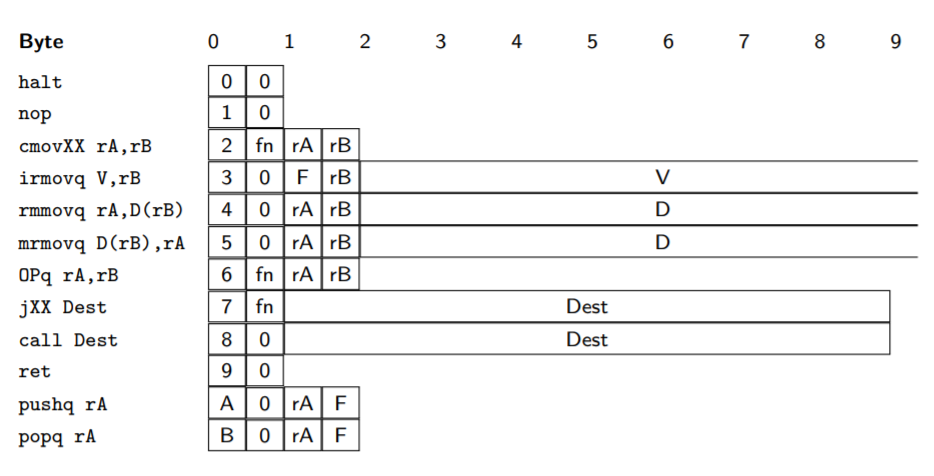
\includegraphics[width=\textwidth]{figures/icodes.png}
    \begin{tabular}{l|c|c||l}
        \hline
        \verb|rrmovq rA, rB|&2&0&Flyt fra register til register\\
        \verb|cmovle rA, rB|&2&1&Flyt hvis mindre eller lig\\
        \verb|cmovl rA, rB|&2&2&Flyt hvis mindre end\\
        \verb|cmove rA, rB|&2&3&Flyt hvis lig med\\
        \verb|cmovne rA, rB|&2&4&Flyt hvis ikke lig\\
        \verb|cmovge rA, rB|&2&5&Flyt hvis større eller lig\\
        \verb|cmovg rA, rB|&2&6&Flyt hvis større end\\\hline
        \verb|addq rA, rB|&6&0&Addition\\
        \verb|subq rA, rB|&6&1&Sutraktion\\
        \verb|andq rA, rB|&6&2&Bitvis AND\\
        \verb|xorq rA, rB|&6&3&Bitvis XOR\\\hline
        \verb|jmp Dest|&7&0&Ikke-konditionelt hop\\
        \verb|jle Dest|&7&1&Hop hvis mindre eller lig\\
        \verb|jl Dest|&7&2&Hop hvis mindre end\\
        \verb|je Dest|&7&3&Hop hvis lig med\\
        \verb|jne Dest|&7&4&Hop hvis ikke lig\\
        \verb|jge Dest|&7&5&Hop hvis større eller lig\\
        \verb|jg Dest|&7&6&Hop hvis større end\\\hline
    \end{tabular}
    \caption{Liste over instruktion- og funktionskoder}
    \label{fig:icode}
\end{figure}
